\documentclass[a4paper]{article}
\usepackage[utf8]{inputenc}
\usepackage[spanish, es-tabla, es-noshorthands]{babel}
\usepackage[table,xcdraw]{xcolor}
\usepackage[a4paper, footnotesep = 1cm, width=20cm, top=2.5cm, height=25cm, textwidth=18cm, textheight=25cm]{geometry}
%\geometry{showframe}

\usepackage{tikz}
\usepackage{amsmath}
\usepackage{amsfonts}
\usepackage{amssymb}
\usepackage{float}
\usepackage{graphicx}
\usepackage{caption}
\usepackage{subcaption}
\usepackage{multicol}
\usepackage{multirow}
\setlength{\doublerulesep}{\arrayrulewidth}
\usepackage{booktabs}

\usepackage{hyperref}
\hypersetup{
    colorlinks=true,
    linkcolor=blue,
    filecolor=magenta,      
    urlcolor=blue,
    citecolor=blue,    
}

\newcommand{\quotes}[1]{``#1''}
\usepackage{array}
\newcolumntype{C}[1]{>{\centering\let\newline\\\arraybackslash\hspace{0pt}}m{#1}}
\usepackage[american]{circuitikz}
\usetikzlibrary{calc}
\usepackage{fancyhdr}
\usepackage{units} 

\graphicspath{{../Ejercicio-1/}{../Ejercicio-2/}{../Ejercicio-3/}{../Ejercicio-4/}}

\pagestyle{fancy}
\fancyhf{}
\lhead{22.01 Teoría de Circuitos}
\rhead{Mechoulam, Lambertucci, Rodriguez Turco, Londero, Galdeman}
\rfoot{\centering \thepage}
\begin{document}

\subsection{Introducción}

En esta sección se implementó un filtro High-Pass utilizando una aproximación \textbf{Cauer} e implementandola con celdas \textbf{Sedra}, el filtro a diseñar deberá cumplir con la siguiente plantilla.
\begin{table}[H]
\centering
\begin{tabular}{|c|c|}
\hline
$f_s$      & 11.65kHz          \\ \hline
$f_p$      & 23.3kHz           \\ \hline
$A_p$      & 2dB               \\ \hline
$A_s$      & 40dB              \\ \hline
$|Z_{in}|$ & $\geq 50k \Omega$ \\ \hline
\end{tabular}
\end{table}
\subsection{Aproximación de Cauer.}
Para esta sección se utlizó la aproximación elíptica de \textbf{Cauer}, además se propuso una plantilla mas restrictiva, con el fin de asegurar el cumplimiento de la original, siendo esta la plantilla final.
\begin{table}[H]
\centering
\begin{tabular}{|c|c|}
\hline
$f_s$      & 11.65kHz          \\ \hline
$f_p$      & 23.3kHz           \\ \hline
$A_p$      & 1dB               \\ \hline
$A_s$      & 45dB              \\ \hline
$|Z_{in}|$ & $\geq 50k \Omega$ \\ \hline
\end{tabular}
\end{table}
Obteniendo la siguiente función transferencia:
\begin{align}
	H(s)=\frac{as^2-bs+c}{(as^2-bs+c)\cdot (as^2-bs+c)}
\end{align}
Y el siguiente diagrama de polos y ceros:
\begin{figure}[H]
	\centering
	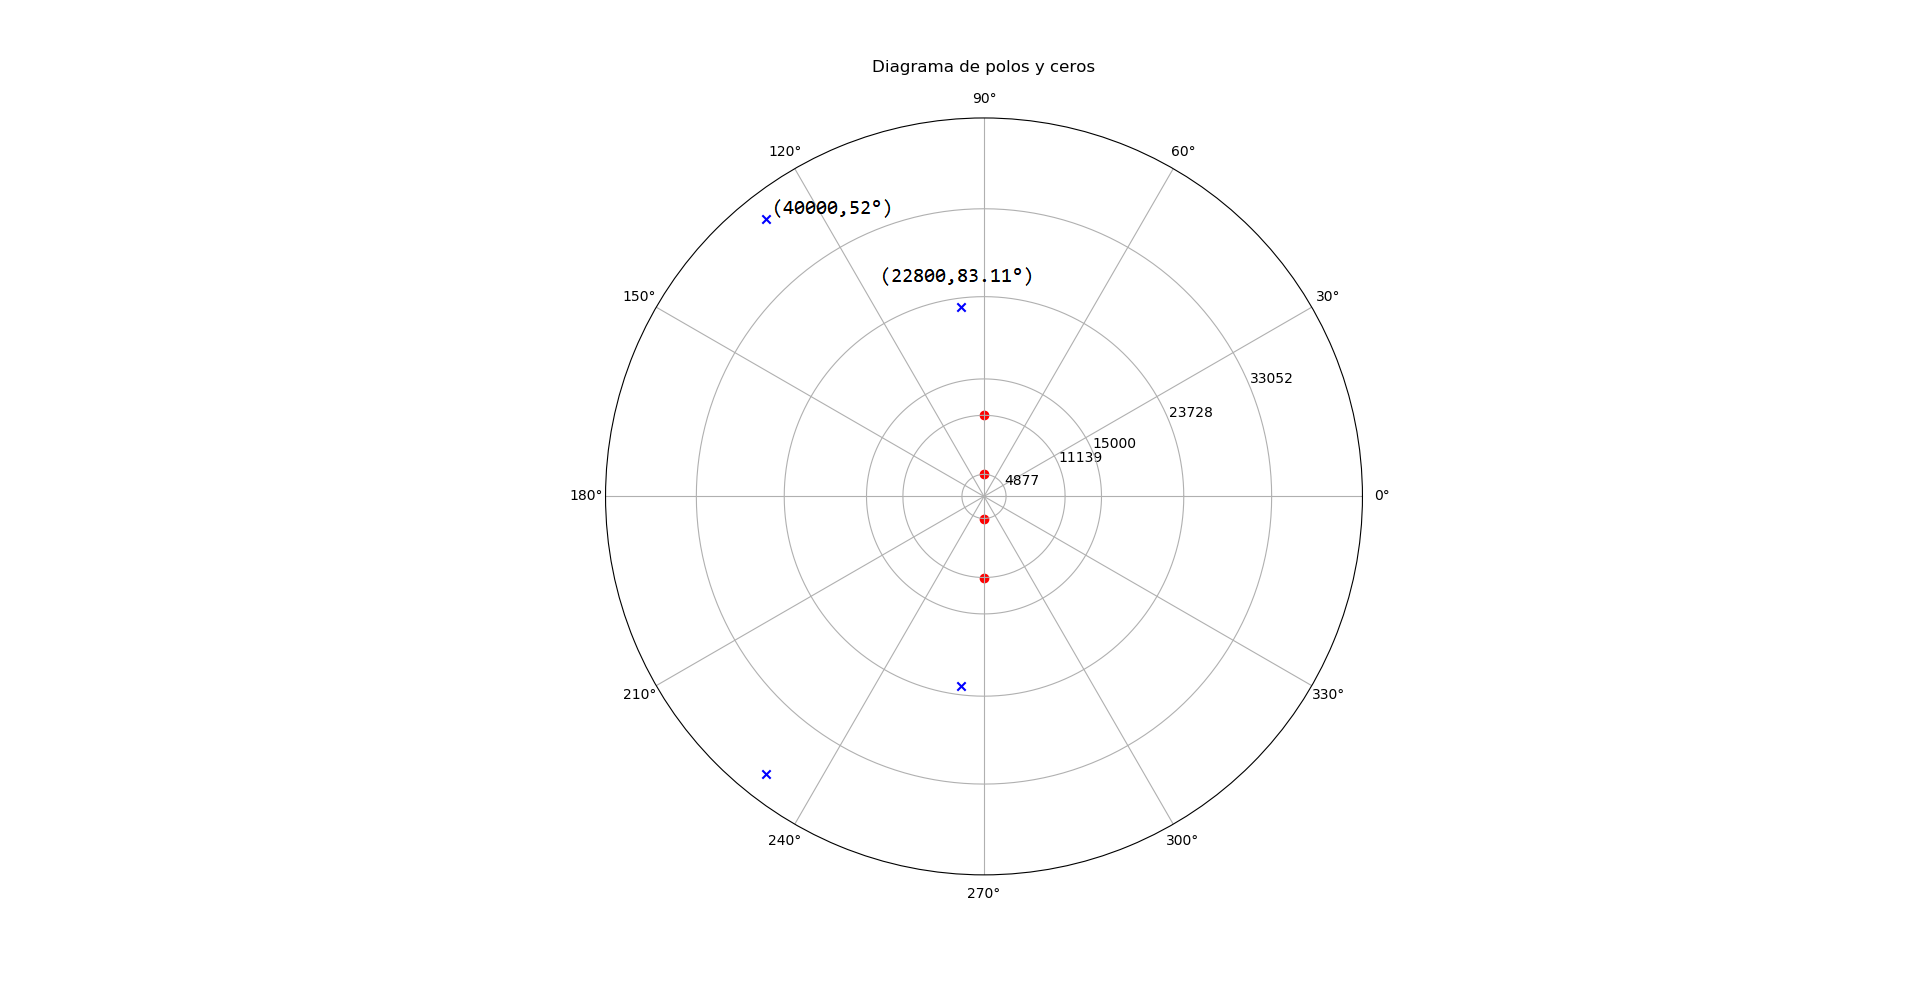
\includegraphics[width=\textwidth]{Imagenes-Ej3/DiagramaPolosYCeros.png}
	\label{fig:stepresponse}
	\caption{Diagrama Polos y Ceros}
\end{figure}

Teniendo los pares de polos con un Q de 0.84 la primer etapa y 4.17.

\subsubsection{Elecciones de diseño}
Se decidió armar etapas con celdas segundo orden en cascada dado a que el orden es 4.
Para la asociación de polos se tomo como criterio agrupar los polos por su cercanía, agrupandolos de las siguiente forma, así mismo la etapa de menor Q será la primera y la de mayor la última.
\subsection{Celda Sedra-Ghorab-Martin.}
La celda Sedra-Ghorab-Martin fue propuesta en el paper ``Optimum Configurations for Single Amplifiers Biquadratic Filters'' como un diseño que permite con un único amplificador operacional (Por eso son llamados Single-Amplifier-Biquad), sintetizar celdas de segundo orden con Q relativamente altos, originalmente esta celda fue propuesta como una mejora de la celda Deliyannis.
Finalmente en el paper discutido se tomó la configuración de HPB dado a que es lo único que utlizaremos, siendo este el circuito propuesto por el paper.
\begin{figure}[H]
	\centering
	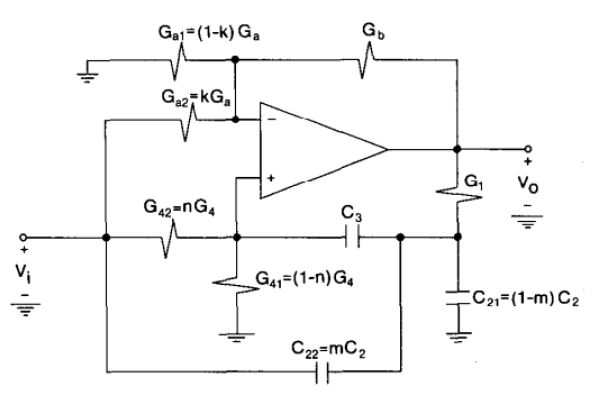
\includegraphics[width=0.5\textwidth]{Imagenes-Ej3/HPBSedra.PNG}
	\label{fig:HPBSedra}
	\caption{Circuito celda SGB-HPB}
\end{figure}
\subsubsection{Cálculo Analítico}
---
\subsubsection{Elecciones de diseño}
El análisis de sensibilidades que se obtiene del circuito, el cual coincide con lo publicado en el paper es la siguiente: 
\begin{center}
	\huge{\textcolor{red}{\textbf{Tabla sensibilidades}}}
\end{center}
En base a esta tabla se tomo especial cuidado en la elección de componentes y en el matcheo de impedancias.
Se tomaron como valor de los componentes los presentados en la siguiente tabla:
\begin{table}[H]
\centering
\begin{tabular}{lllll}
\multicolumn{1}{c}{Componente} & \multicolumn{1}{c}{1er Etapa} & \multicolumn{1}{c}{Composición} & 2da Etapa        & Composición            \\ \hline
$R_1$                          & 12.36k $\Omega$               & 330+12k $\Omega$                & 6.2k $\Omega$    & 1.5k + 4.7k $\Omega$   \\
$R_2$                          & 100k $\Omega$                 & 100k $\Omega$                   & 89.67 k $\Omega$ & 22k + 68k $\Omega$     \\
$R_3$                          & 50.72 k $\Omega$              & 3.9k + 47k $\Omega$             & 1k$\Omega$       & 1k$\Omega$             \\
$R_4$                          & 23.88k $\Omega$               & 1.8k+22k $\Omega$               & 203.36k $\Omega$ & 270k // 820 k $\Omega$ \\
$R_5$                          & 207k $\Omega$                 & 27k + 180k $\Omega$             & 4.19 M$\Omega$   & 1.8M + 2.2M $\Omega$   \\
$R_6$                          & 74.05k $\Omega$               & 18k + 56k $\Omega$              & 25.07k $\Omega$  & 10k+15k $\Omega$       \\
$C_1$                          & 100 pF                        & 100 pF                          & 100 pF           & 100 pF                 \\
$C_2$                          & 74.14 pF                      & 18p // 56p F                    & 18.52p F         & 22pF + 120pF           \\
$C_2$                          & 25.86pF                       & 33p + 120p F                    & 81.48pF          & 82pF+12nF             
\end{tabular}
\end{table}


Se calculó el error porcentual asociado a la aproximación de la resistencias viendose en la siguiente tabla.
\begin{table}[H]
\centering
\begin{tabular}{lll}
\multicolumn{1}{c}{Error Porcentual} & \multicolumn{1}{c}{1er Etapa} & \multicolumn{1}{c}{2da Etapa} \\ \hline
$R_1$                                & 0.2 $\%$                      & $\approx 0 \%$                \\
$R_2$                                & $\approx 0 \%$                & 0.4 $\%$                      \\
$R_3$                                & 0.4 $\%$                      & $\approx 0 \%$                \\
$R_4$                                & 0.3 $\%$                      & 0.1 $\%$                      \\
$R_5$                                & $\approx 0 \%$                & 0.3 $\%$                      \\
$R_6$                                & 0.1 $\%$                      & 0.3 $\%$                      \\
$C_1$                                & $\approx 0 \%$                & $\approx 0 \%$                \\
$C_2$                                & 0.2 $\%$                      & 0.4 $\%$                      \\
$C_2$                                & 0.1 $\%$                      & 0.1 $\%$                     
\end{tabular}
\end{table}

Un criterio utilizado fue tomar capacitores pequeños dado a que ellos son mas certeros y no varían tanto frente a la temperatura.  

\subsubsection{Acoplamiento de Impedancias.}
Para que ambas etapas no se carguen entre si la impedancia de entrada de la segunda etapa debe ser mucho mayor a la de salida de la primera
Asi se simuló la impedancia de entrada de ambas etapas obteniendo las siguientes gráficas:
\begin{figure}[H]
	\centering
	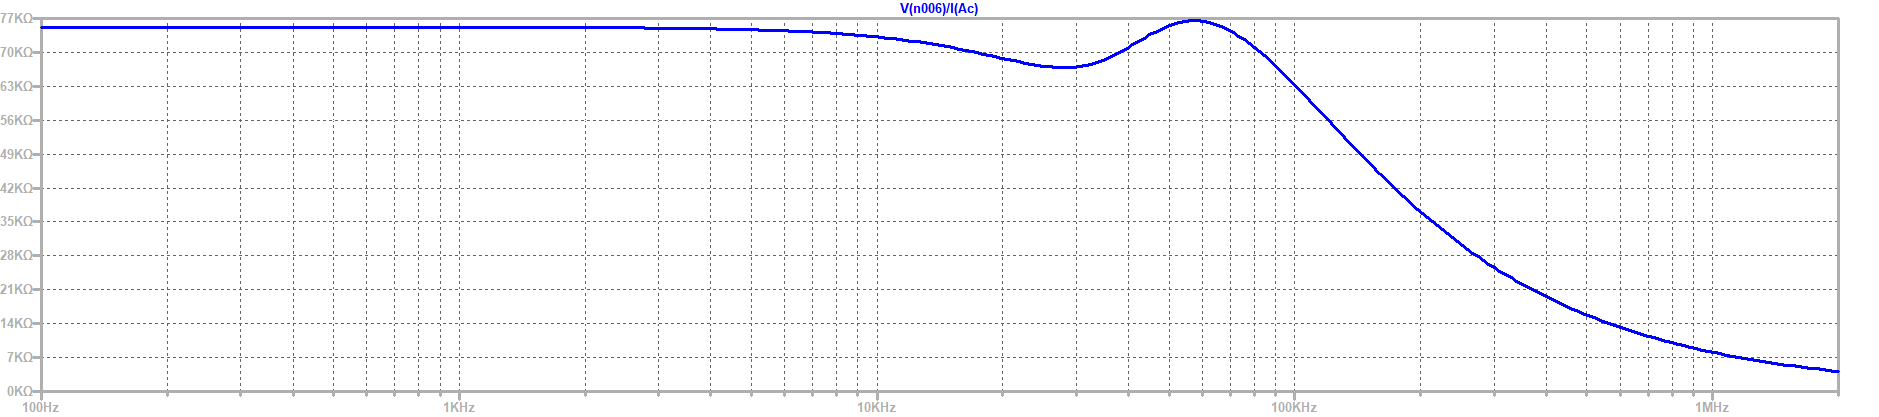
\includegraphics[width=\textwidth]{Imagenes-Ej3/ZinE1.png}
	\label{fig:stepresponse}
	\caption{Impedancia de entrada 1ra etapa}
\end{figure}

\begin{figure}[H]
	\centering
	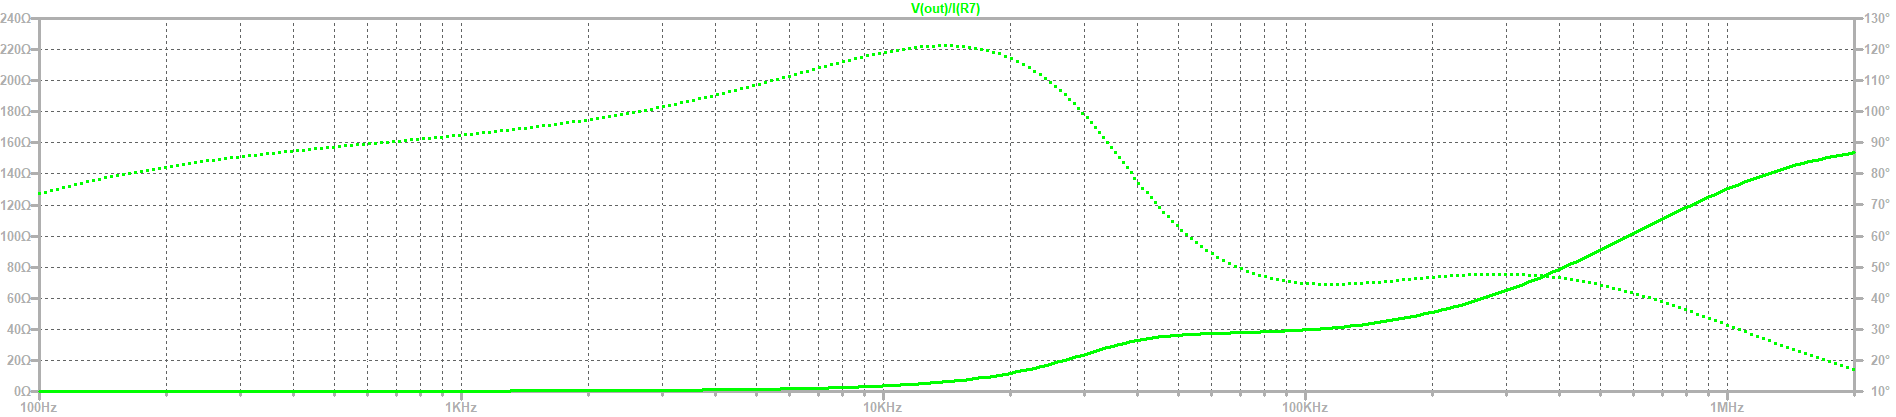
\includegraphics[width=\textwidth]{Imagenes-Ej3/ZoutE1.png}
	\label{fig:stepresponse}
	\caption{Impedancia de salida 1ra etapa}
\end{figure}

\begin{figure}[H]
	\centering
	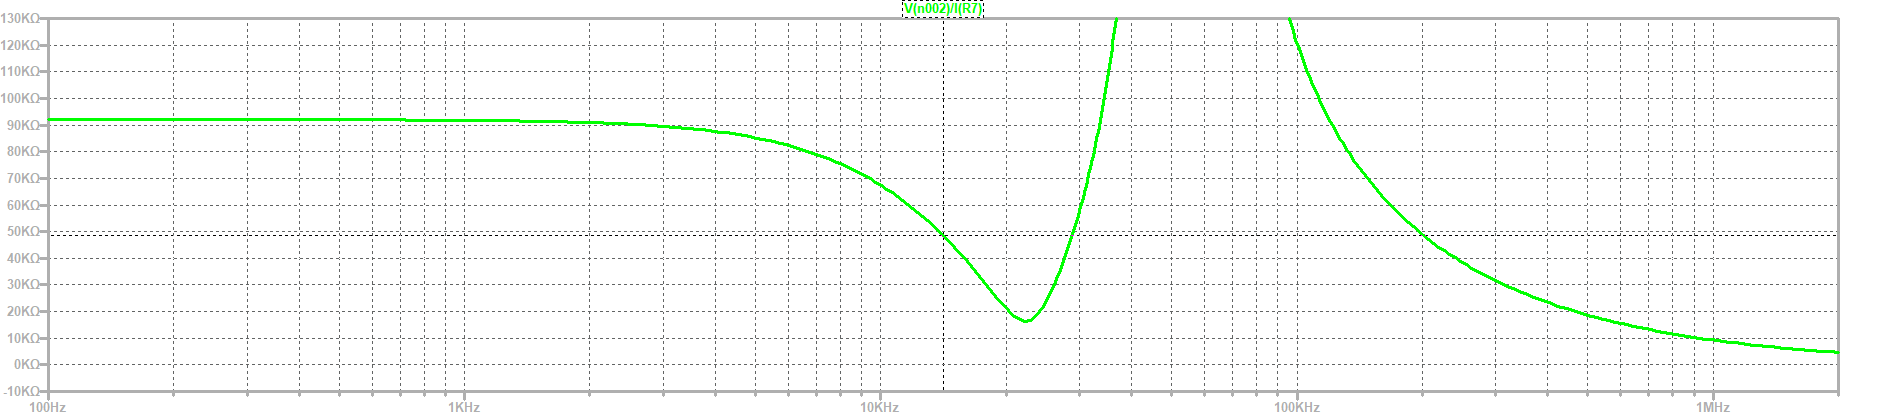
\includegraphics[width=\textwidth]{Imagenes-Ej3/ZinE2.png}
	\label{fig:stepresponse}
	\caption{Impedancia de entrada 2da etapa}
\end{figure}
Se puede concluir luego de estas gráficas que el acoplamiento de impedancias se dará.
\subsection{Respuesta en Frecuencia.}
Se realizó un análisis de Montecarlo a la respuesta en frecuencia del circuito, utilizando una tolerancia de las resistencias al 1$\%$ y capacitores al 10$\%$ obteniendo la siguiente disperción
\begin{figure}[H]
	\centering
	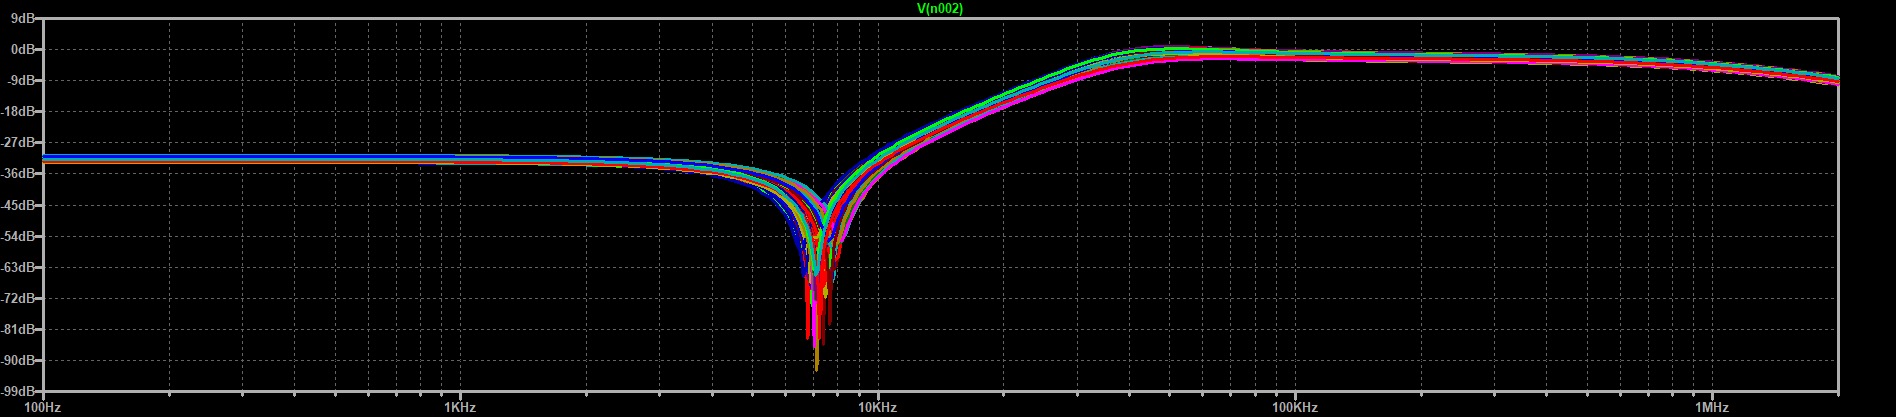
\includegraphics[width=\textwidth]{Imagenes-Ej3/mcsedra.png}
	\label{fig:mcsedra}
\end{figure}

\subsubsection{Filtro definitivo.}
Se realizó el filtro obteniendo la siguiente respuesta en frecuencia 
\begin{figure}[H]
	\centering
	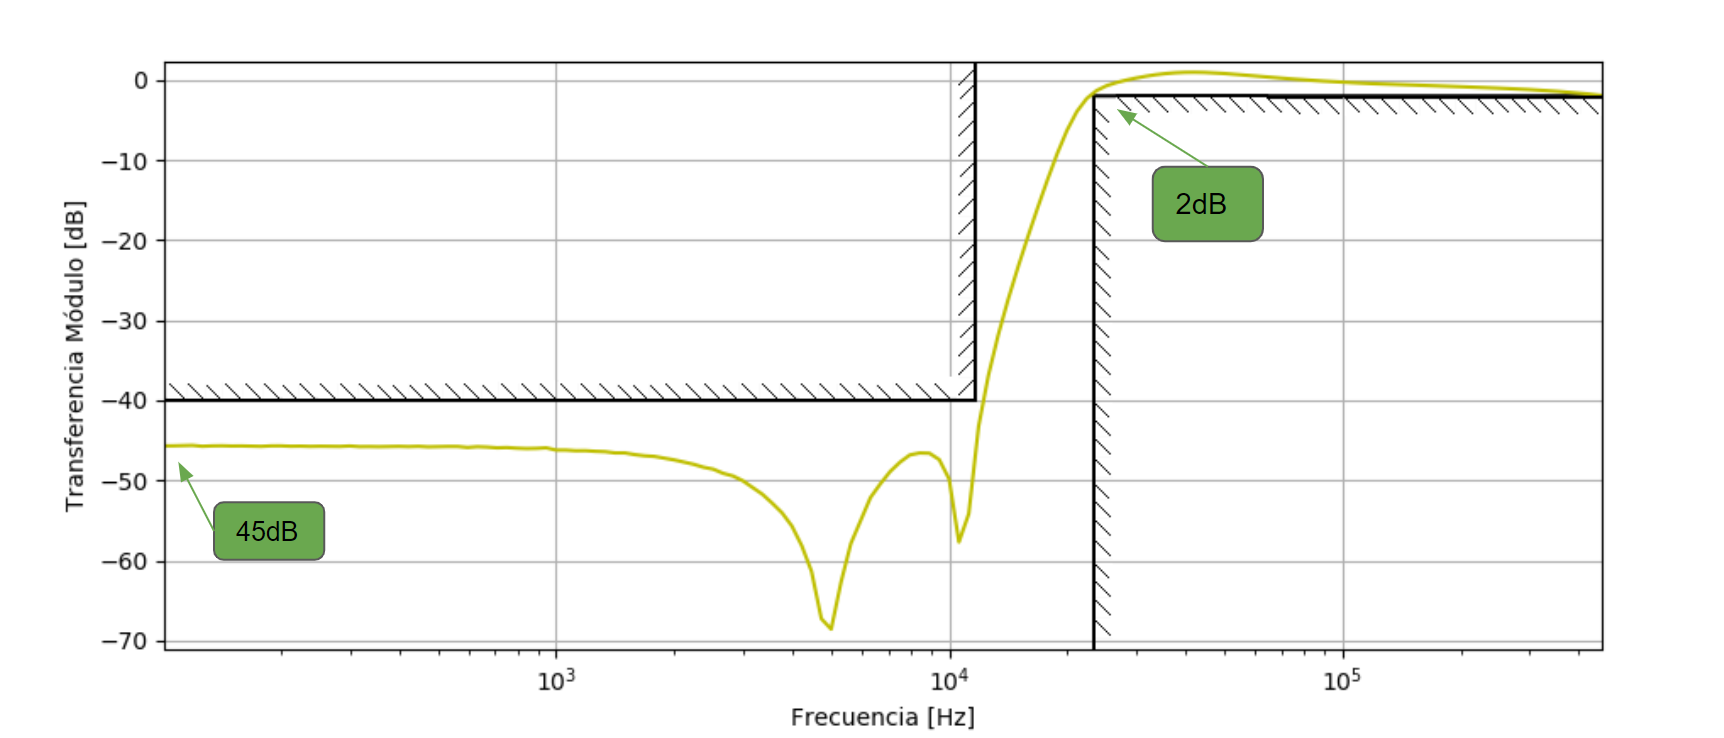
\includegraphics[width=\textwidth]{Imagenes-Ej3/BodeSedra.png}
	\label{fig:BodeSedra}
	\caption{Filtro High-Pass Módulo}
\end{figure}
\begin{figure}[H]
	\centering
	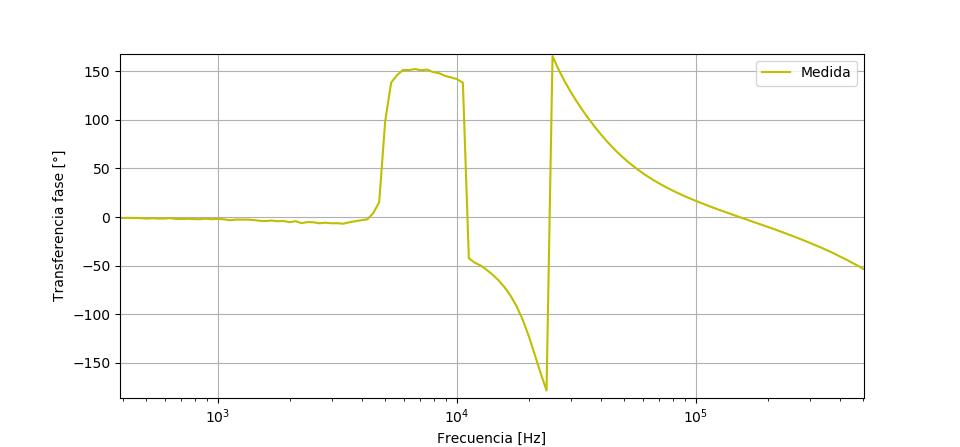
\includegraphics[width=\textwidth]{Imagenes-Ej3/FaseBodeSedra.png}
	\label{fig:FaseBodeSedra}
	\caption{Filtro High-Pass Fase}
\end{figure}
Es de valor apreciar el hecho de que se cumple la plantilla
\subsection{Estabilidad.}
Se intentó en esta sección lograr que la celda oscile, introduciéndole una cuadrada la cual es sabido esta compuesta por un gran numero de frecuencias, asi tambien variando no solo la amplitud de la misma sino tambien su frecuencia y duty-cycle, sin poder hacer osclilar a la celda. La siguietne imagen es la respuesta de la celda al escalón.
\begin{figure}[H]
	\centering
	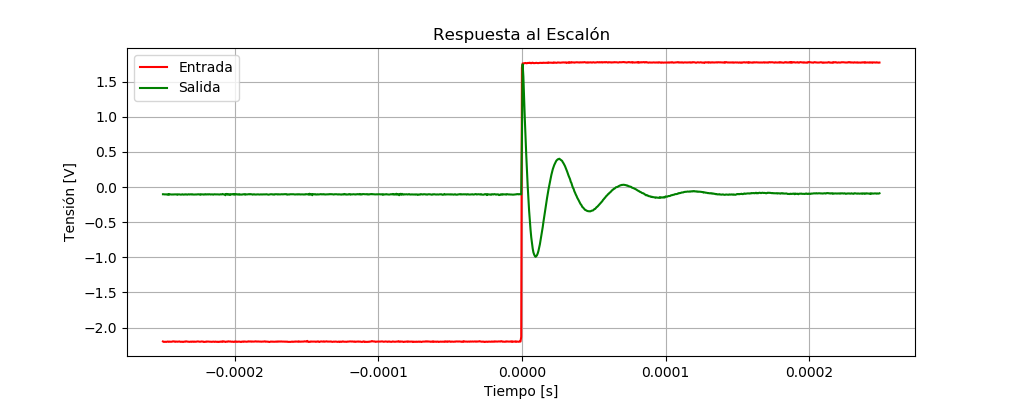
\includegraphics[width=\textwidth]{Imagenes-Ej3/Step.png}
	\label{fig:stepresponse}
	\caption{Respuesta al escalón}
\end{figure}
%
%\begin{figure}[H]
%	\centering
%	\includegraphics[width=0.4\textwidth]{/ImagenesEjercicio3/Graph.png}
%	\label{fig:graph}
%\end{figure}

\end{document}